\documentclass[14pt]{extbook}
\usepackage{multicol, enumerate, enumitem, hyperref, color, soul, setspace, parskip, fancyhdr} %General Packages
\usepackage{amssymb, amsthm, amsmath, bbm, latexsym, units, mathtools} %Math Packages
\everymath{\displaystyle} %All math in Display Style
% Packages with additional options
\usepackage[headsep=0.5cm,headheight=12pt, left=1 in,right= 1 in,top= 1 in,bottom= 1 in]{geometry}
\usepackage[usenames,dvipsnames]{xcolor}
\usepackage{dashrule}  % Package to use the command below to create lines between items
\newcommand{\litem}[1]{\item#1\hspace*{-1cm}\rule{\textwidth}{0.4pt}}
\pagestyle{fancy}
\lhead{Makeup Progress Quiz 1}
\chead{}
\rhead{Version A}
\lfoot{6018-3080}
\cfoot{}
\rfoot{Spring 2021}
\begin{document}

\begin{enumerate}
\litem{
Graph the equation below.\[ f(x) = (x-1)^2 - 15 \]\begin{enumerate}[label=\Alph*.]
\begin{multicols}{2}\item 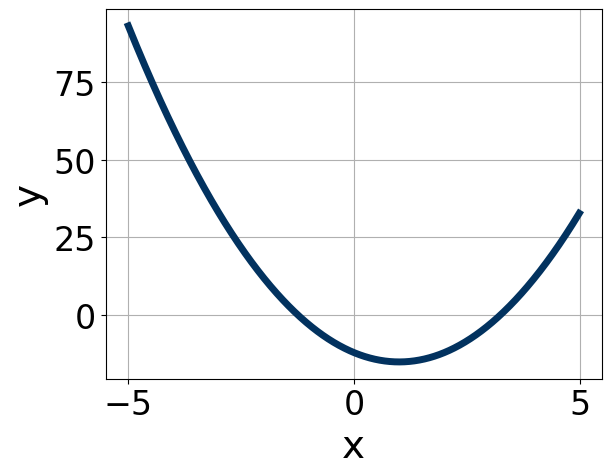
\includegraphics[width = 0.3\textwidth]{../Figures/quadraticEquationToGraphAA.png}\item 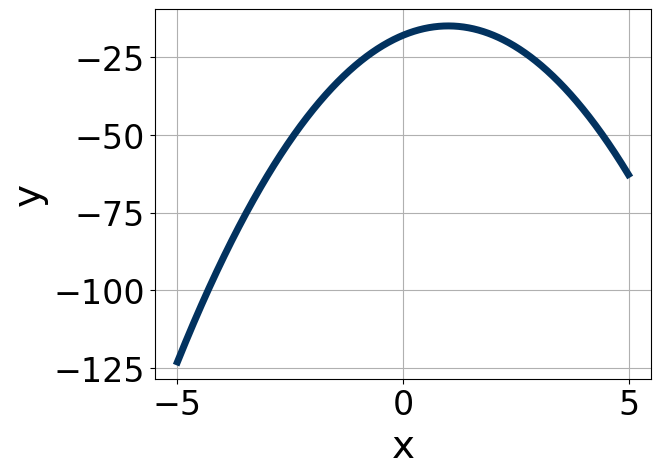
\includegraphics[width = 0.3\textwidth]{../Figures/quadraticEquationToGraphBA.png}\item 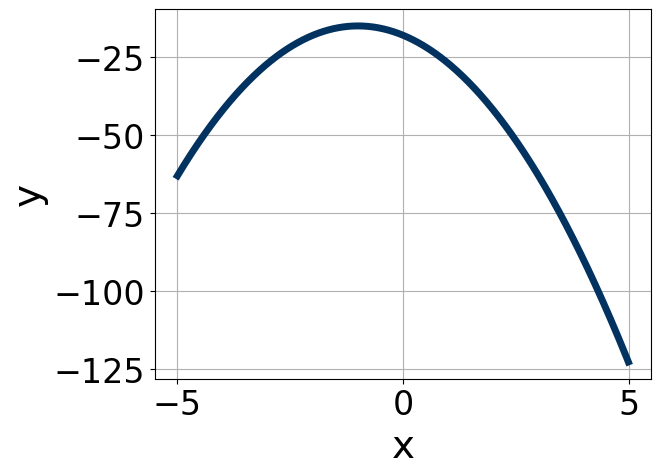
\includegraphics[width = 0.3\textwidth]{../Figures/quadraticEquationToGraphCA.png}\item 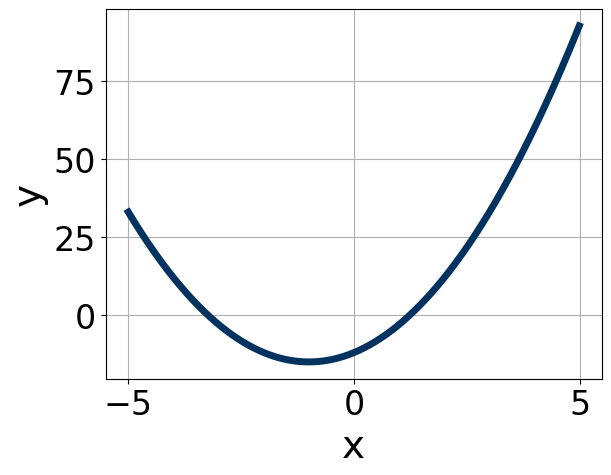
\includegraphics[width = 0.3\textwidth]{../Figures/quadraticEquationToGraphDA.png}\end{multicols}\item None of the above.
\end{enumerate} }
\litem{
Write the equation of the graph presented below in the form $f(x)=ax^2+bx+c$, assuming  $a=1$ or $a=-1$. Then, choose the intervals that $a, b,$ and $c$ belong to.
\begin{center}
    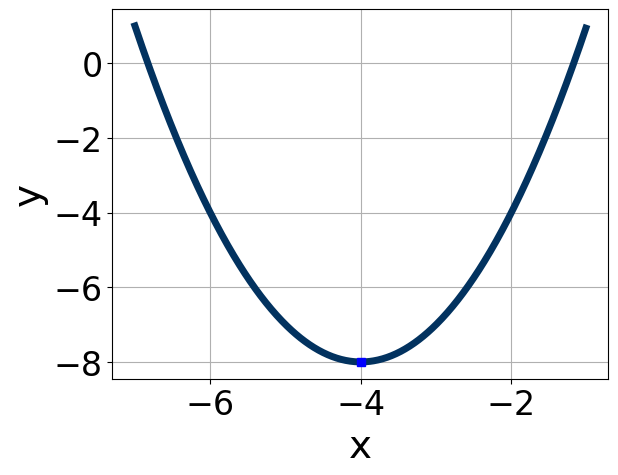
\includegraphics[width=0.5\textwidth]{../Figures/quadraticGraphToEquationCopyA.png}
\end{center}
\begin{enumerate}[label=\Alph*.]
\item \( a \in [-0.4, 1.6], \hspace*{5mm} b \in [-9, -4], \text{ and } \hspace*{5mm} c \in [8, 12] \)
\item \( a \in [-0.4, 1.6], \hspace*{5mm} b \in [7, 10], \text{ and } \hspace*{5mm} c \in [8, 12] \)
\item \( a \in [-1.7, -0.1], \hspace*{5mm} b \in [-9, -4], \text{ and } \hspace*{5mm} c \in [-24, -23] \)
\item \( a \in [-1.7, -0.1], \hspace*{5mm} b \in [7, 10], \text{ and } \hspace*{5mm} c \in [-24, -23] \)
\item \( a \in [-0.4, 1.6], \hspace*{5mm} b \in [-9, -4], \text{ and } \hspace*{5mm} c \in [23, 27] \)

\end{enumerate} }
\litem{
Solve the quadratic equation below. Then, choose the intervals that the solutions belong to, with $x_1 \leq x_2$ (if they exist).\[ 12x^{2} +13 x -2 = 0 \]\begin{enumerate}[label=\Alph*.]
\item \( x_1 \in [-1.6, -0.2] \text{ and } x_2 \in [-0.26, 0.36] \)
\item \( x_1 \in [-15.3, -13.8] \text{ and } x_2 \in [1.47, 1.92] \)
\item \( x_1 \in [-19.2, -16.7] \text{ and } x_2 \in [15.19, 15.93] \)
\item \( x_1 \in [-0.5, 1] \text{ and } x_2 \in [0.82, 1.51] \)
\item \( \text{There are no Real solutions.} \)

\end{enumerate} }
\litem{
Write the equation of the graph presented below in the form $f(x)=ax^2+bx+c$, assuming  $a=1$ or $a=-1$. Then, choose the intervals that $a, b,$ and $c$ belong to.
\begin{center}
    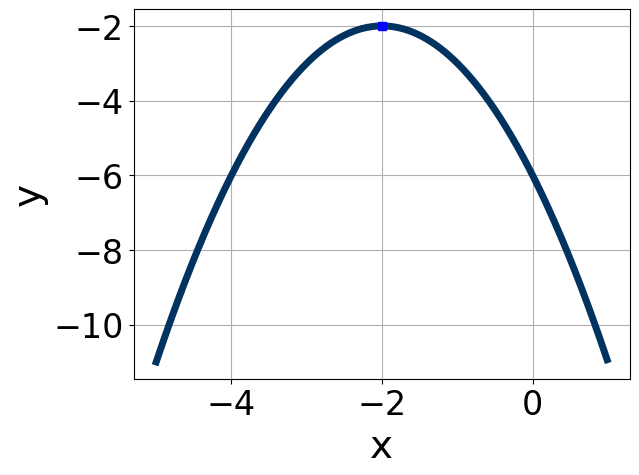
\includegraphics[width=0.5\textwidth]{../Figures/quadraticGraphToEquationA.png}
\end{center}
\begin{enumerate}[label=\Alph*.]
\item \( a \in [-3.7, 0.2], \hspace*{5mm} b \in [-6, -2], \text{ and } \hspace*{5mm} c \in [-7, -4] \)
\item \( a \in [-3.7, 0.2], \hspace*{5mm} b \in [4, 5], \text{ and } \hspace*{5mm} c \in [-7, -4] \)
\item \( a \in [0.5, 1.7], \hspace*{5mm} b \in [4, 5], \text{ and } \hspace*{5mm} c \in [-1, 4] \)
\item \( a \in [-3.7, 0.2], \hspace*{5mm} b \in [4, 5], \text{ and } \hspace*{5mm} c \in [-3, -1] \)
\item \( a \in [0.5, 1.7], \hspace*{5mm} b \in [-6, -2], \text{ and } \hspace*{5mm} c \in [-1, 4] \)

\end{enumerate} }
\litem{
Solve the quadratic equation below. Then, choose the intervals that the solutions $x_1$ and $x_2$ belong to, with $x_1 \leq x_2$.\[ 15x^{2} +8 x -16 = 0 \]\begin{enumerate}[label=\Alph*.]
\item \( x_1 \in [-1.6, -1.02] \text{ and } x_2 \in [0.75, 0.81] \)
\item \( x_1 \in [-4.63, -3.81] \text{ and } x_2 \in [0.18, 0.28] \)
\item \( x_1 \in [-0.83, -0.34] \text{ and } x_2 \in [1.42, 1.63] \)
\item \( x_1 \in [-3.17, -2.18] \text{ and } x_2 \in [0.34, 0.45] \)
\item \( x_1 \in [-20.03, -18.91] \text{ and } x_2 \in [11.89, 12.11] \)

\end{enumerate} }
\litem{
Graph the equation below.\[ f(x) = (x-2)^2 - 10 \]\begin{enumerate}[label=\Alph*.]
\begin{multicols}{2}\item 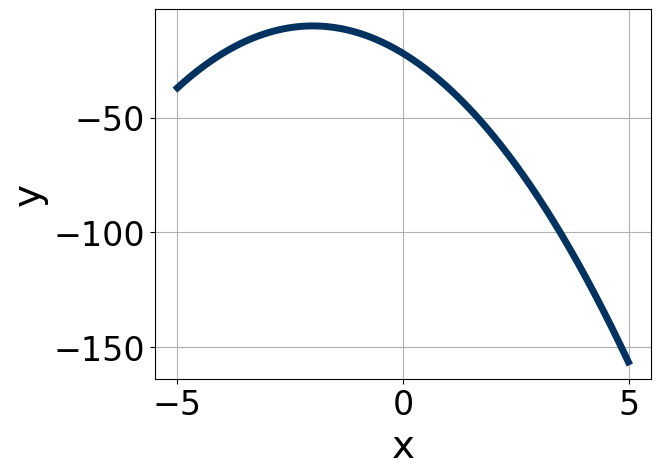
\includegraphics[width = 0.3\textwidth]{../Figures/quadraticEquationToGraphCopyAA.png}\item 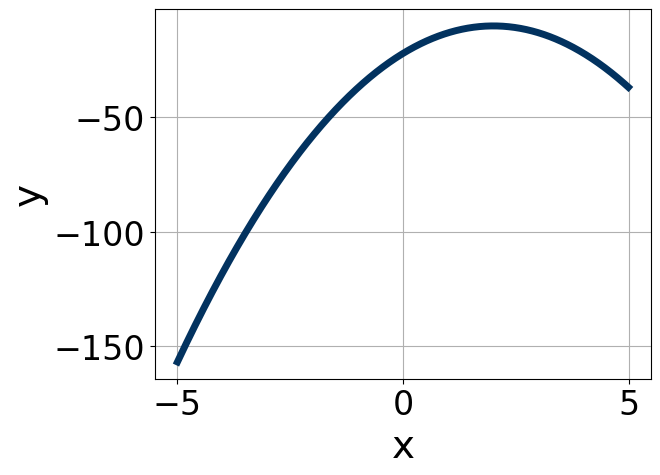
\includegraphics[width = 0.3\textwidth]{../Figures/quadraticEquationToGraphCopyBA.png}\item 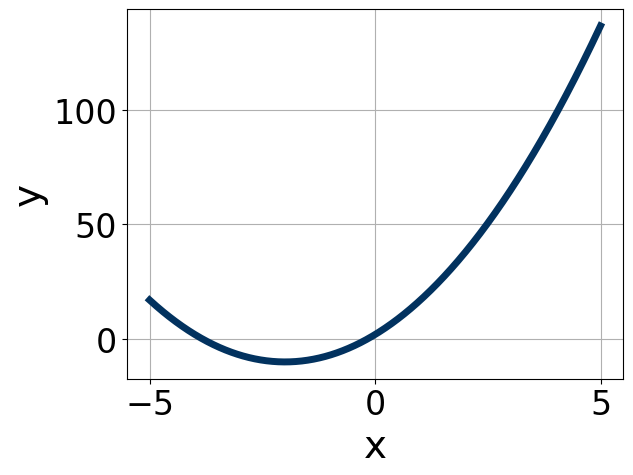
\includegraphics[width = 0.3\textwidth]{../Figures/quadraticEquationToGraphCopyCA.png}\item 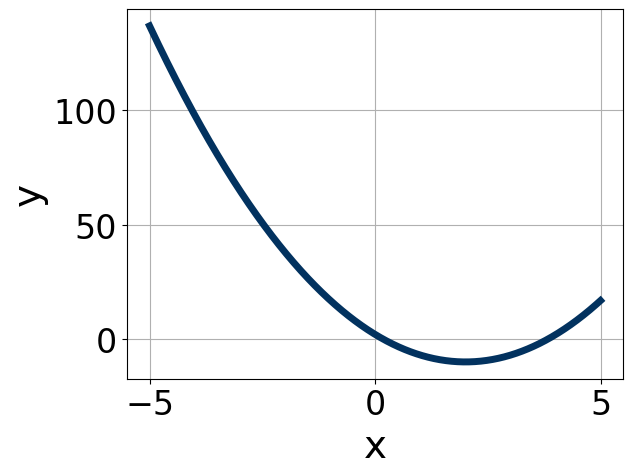
\includegraphics[width = 0.3\textwidth]{../Figures/quadraticEquationToGraphCopyDA.png}\end{multicols}\item None of the above.
\end{enumerate} }
\litem{
Factor the quadratic below. Then, choose the intervals that contain the constants in the form $(ax+b)(cx+d); b \leq d.$\[ 36x^{2} +60 x + 25 \]\begin{enumerate}[label=\Alph*.]
\item \( a \in [11.98, 13.44], \hspace*{5mm} b \in [0, 7], \hspace*{5mm} c \in [2.63, 3.3], \text{ and } \hspace*{5mm} d \in [4, 7] \)
\item \( a \in [5.89, 6.22], \hspace*{5mm} b \in [0, 7], \hspace*{5mm} c \in [5.93, 6.28], \text{ and } \hspace*{5mm} d \in [4, 7] \)
\item \( a \in [0.79, 1.62], \hspace*{5mm} b \in [25, 38], \hspace*{5mm} c \in [0.75, 1.3], \text{ and } \hspace*{5mm} d \in [22, 35] \)
\item \( a \in [1.44, 2.64], \hspace*{5mm} b \in [0, 7], \hspace*{5mm} c \in [16.62, 18.14], \text{ and } \hspace*{5mm} d \in [4, 7] \)
\item \( \text{None of the above.} \)

\end{enumerate} }
\litem{
Solve the quadratic equation below. Then, choose the intervals that the solutions $x_1$ and $x_2$ belong to, with $x_1 \leq x_2$.\[ 10x^{2} +33 x -54 = 0 \]\begin{enumerate}[label=\Alph*.]
\item \( x_1 \in [-12.3, -8.6] \text{ and } x_2 \in [0.48, 0.64] \)
\item \( x_1 \in [-14.8, -10.5] \text{ and } x_2 \in [0.2, 0.51] \)
\item \( x_1 \in [-2, 0.9] \text{ and } x_2 \in [3.53, 3.92] \)
\item \( x_1 \in [-45.2, -43.1] \text{ and } x_2 \in [11.9, 12.08] \)
\item \( x_1 \in [-5.8, -4.4] \text{ and } x_2 \in [0.98, 1.47] \)

\end{enumerate} }
\litem{
Solve the quadratic equation below. Then, choose the intervals that the solutions belong to, with $x_1 \leq x_2$ (if they exist).\[ 14x^{2} -10 x -9 = 0 \]\begin{enumerate}[label=\Alph*.]
\item \( x_1 \in [-7.7, -5.8] \text{ and } x_2 \in [16.82, 17.78] \)
\item \( x_1 \in [-25.4, -22.8] \text{ and } x_2 \in [24.71, 25.49] \)
\item \( x_1 \in [-2.9, -0.8] \text{ and } x_2 \in [-0.4, 0.6] \)
\item \( x_1 \in [-1.2, 0.6] \text{ and } x_2 \in [0.84, 1.41] \)
\item \( \text{There are no Real solutions.} \)

\end{enumerate} }
\litem{
Factor the quadratic below. Then, choose the intervals that contain the constants in the form $(ax+b)(cx+d); b \leq d.$\[ 16x^{2} -8 x -15 \]\begin{enumerate}[label=\Alph*.]
\item \( a \in [1.34, 2.46], \hspace*{5mm} b \in [-5, -3], \hspace*{5mm} c \in [6.68, 8.99], \text{ and } \hspace*{5mm} d \in [1, 7] \)
\item \( a \in [0.33, 1.65], \hspace*{5mm} b \in [-22, -16], \hspace*{5mm} c \in [0.48, 1.14], \text{ and } \hspace*{5mm} d \in [11, 13] \)
\item \( a \in [2.7, 5.54], \hspace*{5mm} b \in [-5, -3], \hspace*{5mm} c \in [3.67, 5.5], \text{ and } \hspace*{5mm} d \in [1, 7] \)
\item \( a \in [6.75, 8.17], \hspace*{5mm} b \in [-5, -3], \hspace*{5mm} c \in [1.65, 2.71], \text{ and } \hspace*{5mm} d \in [1, 7] \)
\item \( \text{None of the above.} \)

\end{enumerate} }
\end{enumerate}

\end{document}